\subsection{Schraubenquerschnitte \hfill ME}
\begin{footnotesize}
    \begin{minipage}{0.55\linewidth}
        \begin{center}
            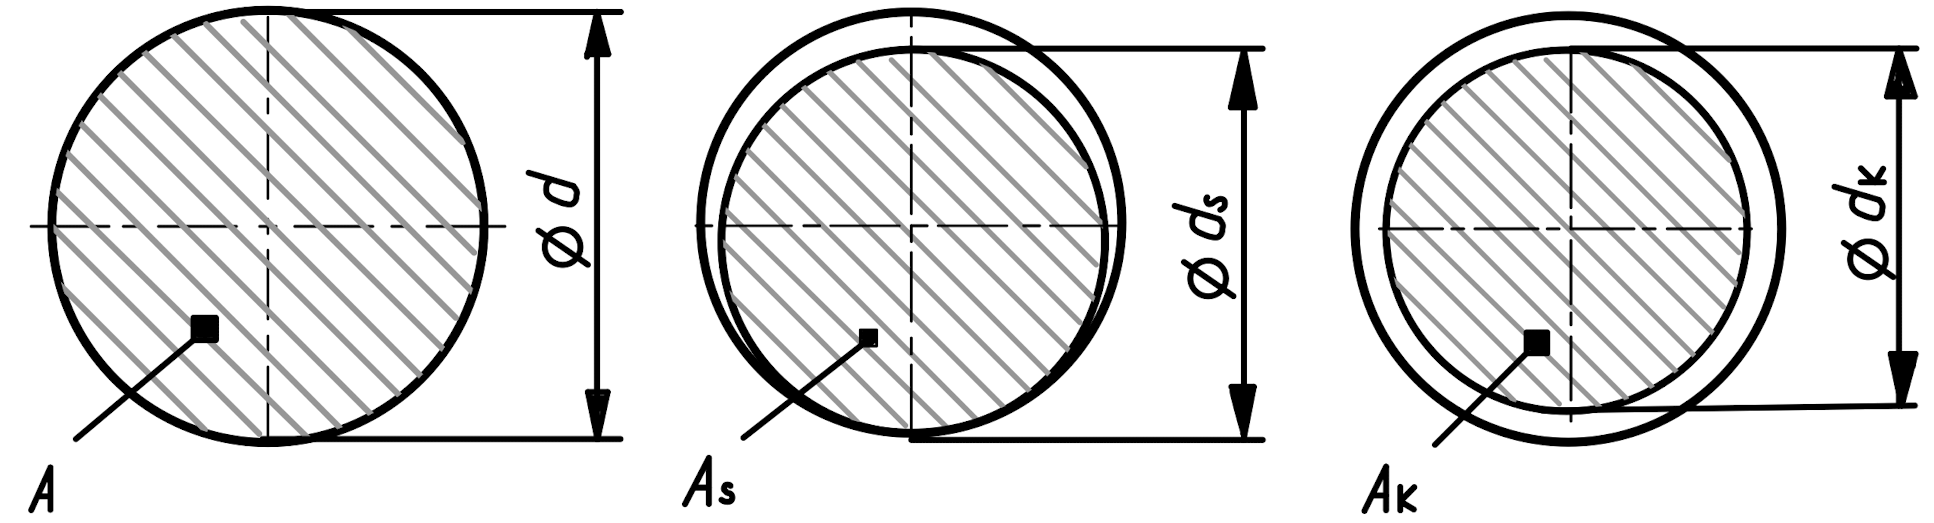
\includegraphics[width = 0.9\linewidth]{src/images/MAEIP_Schraubenquerschnitte}
            \mathbox{
                d_s = \frac{1}{2} \cdot (d_2 + d_3)
            }
        \end{center}
    \end{minipage}
\end{footnotesize}
    \begin{minipage}{0.4\linewidth}
        \begin{scriptsize}
        \begin{center}
            \begin{align*}
                d &= \text{Nenndurchmesser} [d_2]
                \\d_s &= \text{Spannungsdurchmesser}
                \\d_k &= \text{Kerndurchmesser} [d_3]
                \\A &= \text{Schaftquerschnitt} [A_2]
                \\A_s &= \text{Spannungsquerschnitt}
                \\A_k &= \text{Kernquerschnitt} [A_3]
            \end{align*}
        \end{center}
    \end{scriptsize}
    \end{minipage}